\newpage
\texHeader

\subsection{Eclipse and the MOSL structure (Textual)}

As\hypertarget{projectStructure tex}{} you now know, eMoflon is a plug-in tool for Eclipse. More precisely, eMoflon needs the the Eclipse Modeling Framework (EMF) in order to work. EMF is comprised of two separate metamodels - Genmodel and Ecore. The Genmodel contains the boring information about code generation like path and file information. 
We are more interested in Ecore, which we represent through our MOSL syntax. 

When you switched the project explorer from \texttt{Projects} to \texttt{Top Level Elements}, you noticed that a few new nodes were created. Each node you see has a different criteria for grouping related Eclipse Projects together, which makes them your project \emph{working sets}. 

The \texttt{Specifications} working set contains all \emph{metamodel projects} in a workspace (Fig. ~\ref{fig_modelSpecification}). That means, for every new metamodel you create in your current workspace, all of the text code will be placed here.

 \begin{figure}[htbp]
  \centering
  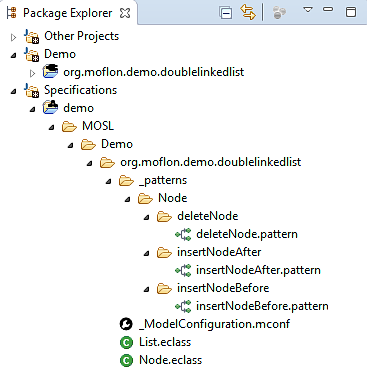
\includegraphics[width=0.5\textwidth]{eclipse_Specification}
  \caption{Eclipse: Specification Working Set}
  \label{fig_modelSpecification}
\end{figure}
  

Lets look at the two \emph{eclass} files. While you can usually combine several short class delcarations in a single file in some languages (like Java), with MOSL it really is best to have them separated. It'll all make sense in a moment when we discuss \emph{patterns}.

Inspect the \texttt{List} eclass, and you'll see it has a just one \emph{EAttribute}. EAttributes are defined by their name, followed by a colon symbol and type. This class also has one type of \emph{EReference}, a \emph{container reference}. This is represented by the diamond operator in front of an arrow. Switch to the \texttt{Node} eclass and you can observe the second reference type, a \emph{simple reference}. It's represented by a plain arrow. EReference names are immediately followed by their multiplicity and then, just like an attribute, a colon and their datatype.

While we're on the topic of syntax, lets have a quick overview on MOSL operators. The \texttt{`@'} before a name represents a bounded variable, \texttt{`--'} shows intended removal (destruction), and the opposite \texttt{`++'} operator signals something to be made (creation). These operators can be placed before directly names or other operators, such as references.  All black items are elements of context, and must exist before and after the control flow. 

Lets go back to looking at the code. In the \texttt{Node} class (Fig.~\ref{fig_patternDeleteNode}), a few methods have been declared. You can see each function is remarkably small. In fact,the only thing the functions are doing are calling patterns. These patterns represent dynamic action within the program, and their container functions are used exclusively for control flow. Don't forget the \texttt{return} command - you can't exit the flow without it. 

 \begin{figure}[htbp]
  \centering
  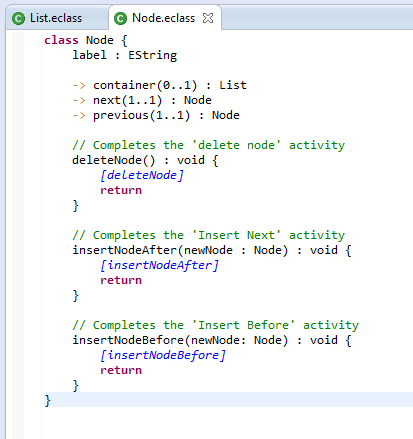
\includegraphics[width=0.6\textwidth]{eclipse_eclassNode}
  \caption{Eclipse: The Node eclass}
  \label{fig_eclassNode}
\end{figure}

Given that the activities are never directly implemented, just where are these pattern defined? And why are they somewhere else? 

After many long discussions, it was decided that patterns must follow a strict, predictable path. Inspect Figure~\ref{fig_modelSpecification} again, and observe the locations where the patterns are stored. You'll notice that there is a folder for the ``Node'' eclass, and a subfolder for each method. There's no folder for ``List'' purely because it never calls a pattern. It is imperative in the future that every pattern created follows this `\texttt{\_pattern}/Class/Method/patternName.pattern' set up.

On a final note, one of the really neat things about EReferences in MOSL is that the other object involved in the relation is automatically updated! Check out the \texttt{deleteNode} pattern (Fig ~\ref{fig_patternDeleteNode}). 

 \begin{figure}[htbp]
  \centering
  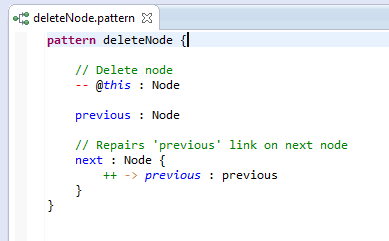
\includegraphics[width=0.6\textwidth]{eclipse_patternDeleteNode}
  \caption{Eclipse: The deleteNode Pattern}
  \label{fig_patternDeleteNode}
\end{figure}

You can see that a creation reference is made from \texttt{next} to \texttt{previous}, but the matching creation reference for \texttt{previous} to \texttt{next} is not. It's simply not needed! MOSL takes care of these automatically which means you'll never have an issue with hanging links. 

This update works for destruction calls as well. You can see that there is a destroy command on \texttt{@this}. It gets rid of the node, but it doesn't do anything about the previous and next references defined on it. That's because when the node is removed, everything attached to it will be cleaned and updated.
 
So that's a quick overview of the MOSL language but again, how to we generate code from all of this?

First, eMoflon does not do a compelete code generation. To improve performance, only the parser and error detection starts when you save files. This means that to build generate the project, we need to press the \texttt{Build (and clean)} command from the eMoflon context menu after right clicking your working set.

\fancyfoot[R]{  $\triangleright$ \hyperlink{codeGen common}{Next Step} }

Second, this is actually where the Eclipse EMF kicks in! The hidden \texttt{.genmodel} metamodel was automatically created, which meant that all we needed to make was the ecore model, which is collectively made of all of our MOSL files. By invoking the \texttt{Build} command above, code generation was initalized and completed. The following section offers a discussion on all of this, as it's virtually the same as its visual counterpart.